\documentclass[11pt,letterpaper,final]{report}
\usepackage[utf8]{inputenc}
\usepackage[francais]{babel}
\usepackage[T1]{fontenc}
\usepackage{amsmath}
\usepackage{amsfonts}
\usepackage{amssymb}
\usepackage{graphicx}
\usepackage{lmodern}
\usepackage[left=2.54cm,right=2.54cm,top=2.54cm,bottom=2.54cm]{geometry}
\begin{document}
\chapter{Cross validation entre les différentes plateformes de simulations}
\section{Validation Psim/SPS}
\begin{figure}[ht]
\centering
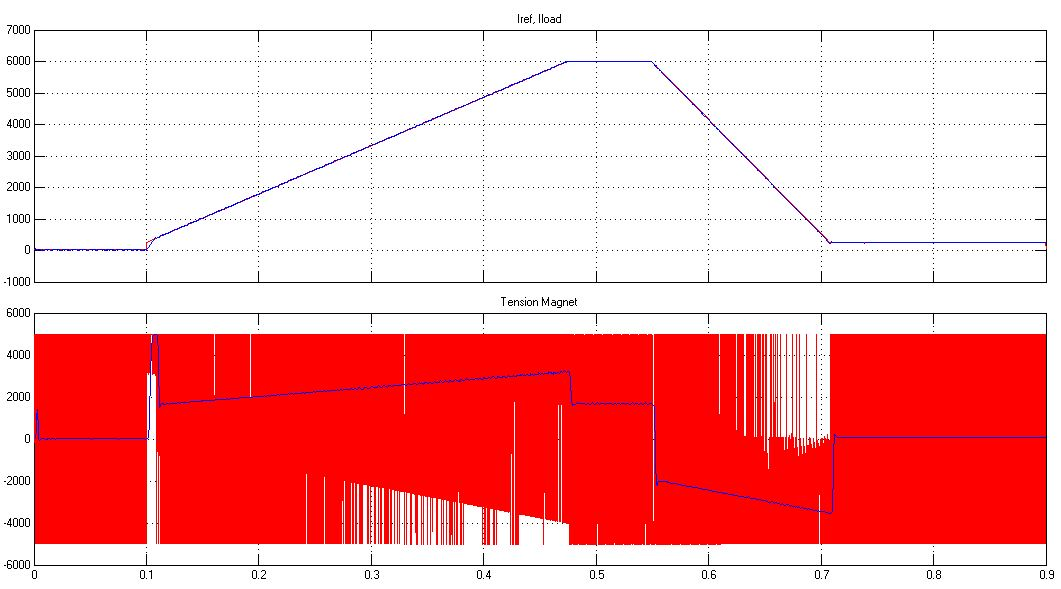
\includegraphics[scale=0.5]{fig/resul_sim.jpg}
\caption{Résultats de simulation sur SIMULINK}
\end{figure}
\begin{figure}[ht]
\centering
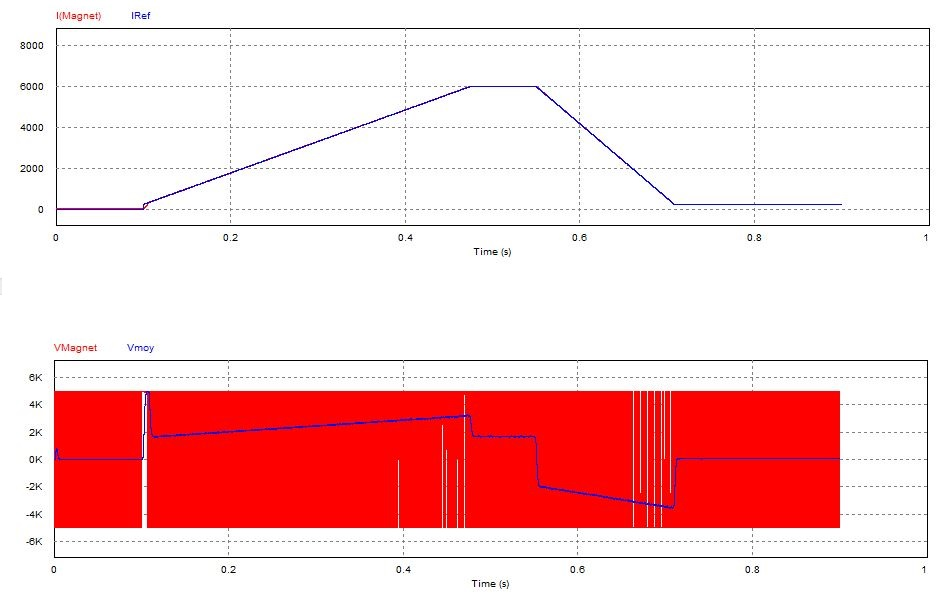
\includegraphics[scale=0.6]{fig/resul_psim.jpg}
\caption{Résultats de simulation sur Psim}
\end{figure}
\subsection{Calcul de la tension moyenne}

Commençons par discuter des différences obtenues entre les différentes simulations. On a remarqué que la fonction "Mean" dans simulink et Psim ne donne pas le même résulat. Pour le montrer, on a testé chacune des deux fonctions avec un sinus 100Vamplitude, 50Vmoy et à 1KHz de fréquence. Les figures~\ref{dis_mean} et \ref{D_mean} montre les résulats obtenus avec une fréquence de 500Hz du moyenneur.



\begin{figure}[h]
\centering
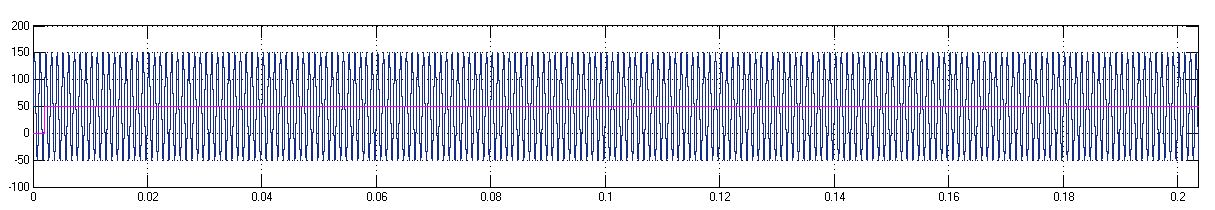
\includegraphics[scale=0.5]{fig/moy_sim.jpg}
\caption{Réponse de la fonction "Discrete Mean" sur SPS}
\label{dis_mean}
\end{figure}

\begin{figure}[h]
\centering
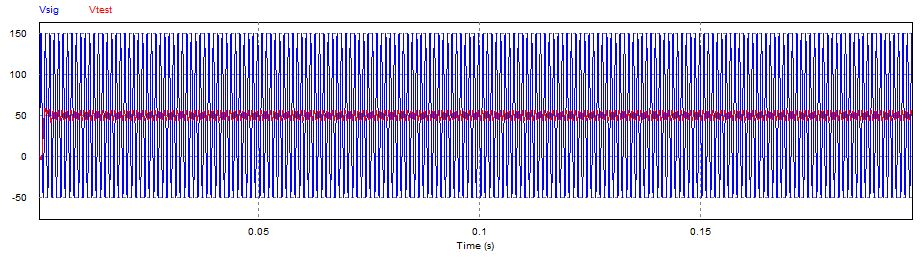
\includegraphics[scale=0.5]{fig/moy_psim.jpg}
\caption{Réponse du bloc "DC Voltmeter" sur PSIM}
\label{D_mean}
\end{figure}


\begin{figure}[ht]
\centering
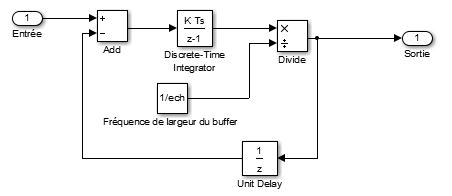
\includegraphics[scale=0.8]{fig/moy.jpg}
\caption{Fonction de moyennage de la tension}
\label{moy}
\end{figure}
On remarque bien que les résultats sont différents dans les figures~\ref{dis_mean} et \ref{D_mean}. La tension moyenne calculé sur simulink est plus précise et varie moins que celle de Psim. La précision est telle que le résultat de Psim est variant sur chaque période tandis que celle de simulink a une apparence droite. Par contre, le temps de réponse de simulink est plus long que celui de Psim. Par conséquent, on a décidé de monter notre propre fonction de moyennage pour avoir un fonctionnement identique dans les deux simulations. La figure~\ref{moy} représente la fonction qui est constitué d'un intégrateur avec un gain unitaire. Cette valeur est passé dans un gain de 3000 qui contrôle la sensibilité du calcul de moyennage. De plus, on a cascadé 10 fonctions de moyennage pour optimiser le résultat et avoir une moyenne avec une oscillation négligeable. Comme les filtres donnent le même résultat sur les deux plateformes donc le fonctionnement de la fonction de moyennage sur Psim est identique et donne le même résultat que celle de Simulink si le signal d'entrée est le même. 




\begin{figure}[h!]
\centering
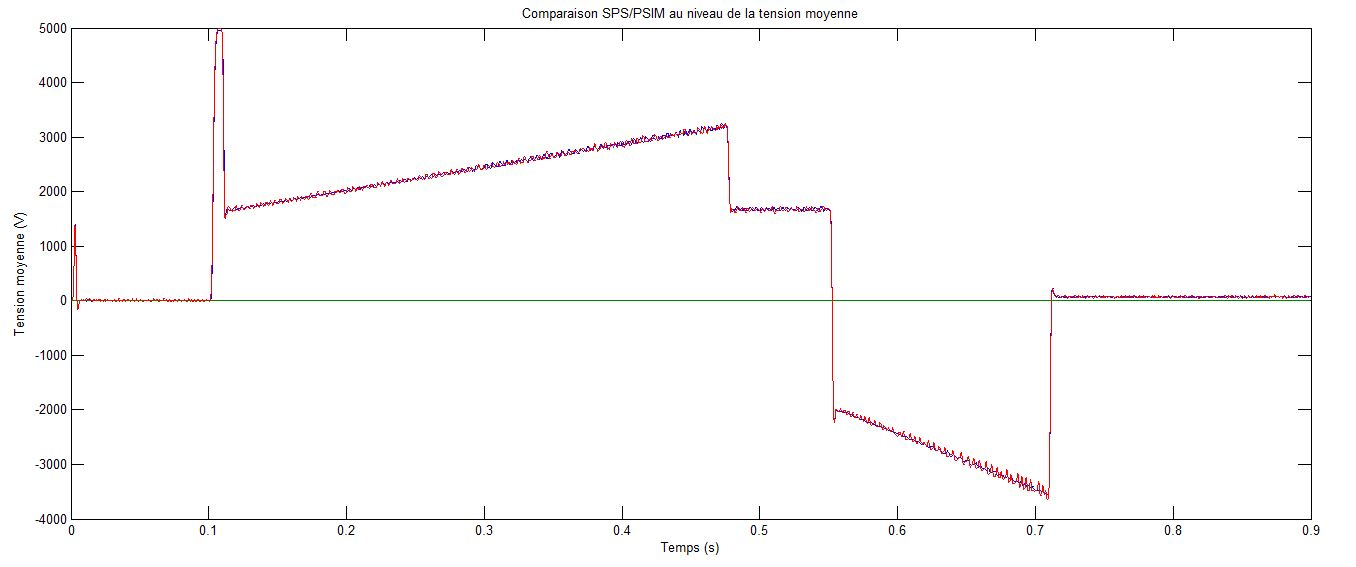
\includegraphics[scale=0.4]{fig/tmoypsim_sim.jpg}
\caption{La tension moyenne Psim/Simulink}
\label{moyt}
\end{figure}
Sur la figure~\ref{moyt} on capte la différence relative entre la tension moyenne sur Psim et Simulink. La courbe en vert représente la réponse sur Psim et en bleu celle sur Simulink. La différence observé est dû au fait que sur Simulink nous utilisons des IGBT idéaux donc qui commutent instantanément, tandis que sur Psim ce sont des IGBT qui ont un temps de commutation faible mais non négligeable. Leur modélisation n'est donc pas pareil. De sorte que, c'est normal qu'on n'ait pas le même résultat car la simulation de Psim a une perte de commutation tandis que celle de Simulink n'en a pas. Par contre, on constate que les résultats sont très semblables avec une erreur moyenne de seulement 0.0358\% calculé selon l'équation~\ref{eq1}. Donc, on déduit que même avec une modélisation différente, le résultat est très semblable. Il faut aussi comprendre que les IGBT de simulink sont plus dévéloppés que ceux de Psim. Ils contiennent un snubber RC intégré, ce qui n'est pas le cas sur Psim. De plus, sur simulink il est possible de mettre la valeur d'un condensateur à inf ce qui représente pour le snubber un fonctionnement purement résistif. Psim ne permet pas de mettre un condensateur à inf, il faut le mettre plutôt à 0 si on veut rajouter des snubber RC au circuit mais avec un fonctionnement R.
\begin{equation}
Erreur = \frac{mean(V_{moy Simulink})-mean(V_{moy Psim})}{mean(V_{moy Simulink})}
\label{eq1}
\end{equation}




\subsection{Calcul du courant}
Nous avons comparés les deux plateformes concernant la différence obtenus au niveau du courant de charge. Nous avons obtenu une différence de 0.0048\%
entre Psim et Simulink en utilisant la valeur moyenne de courant en suivant l'équation~\ref{eq2}. On déduit donc que la simulation de Psim représente le fonctionnement réel du système car il reproduit bien les résultats obtenus sur Simulink.
 
\begin{equation}
Erreur = \frac{mean(I_{simulink})-mean(I_{Psim})}{mean(I_{simulink})}
\label{eq2}
\end{equation}


\begin{figure}[ht]
\centering
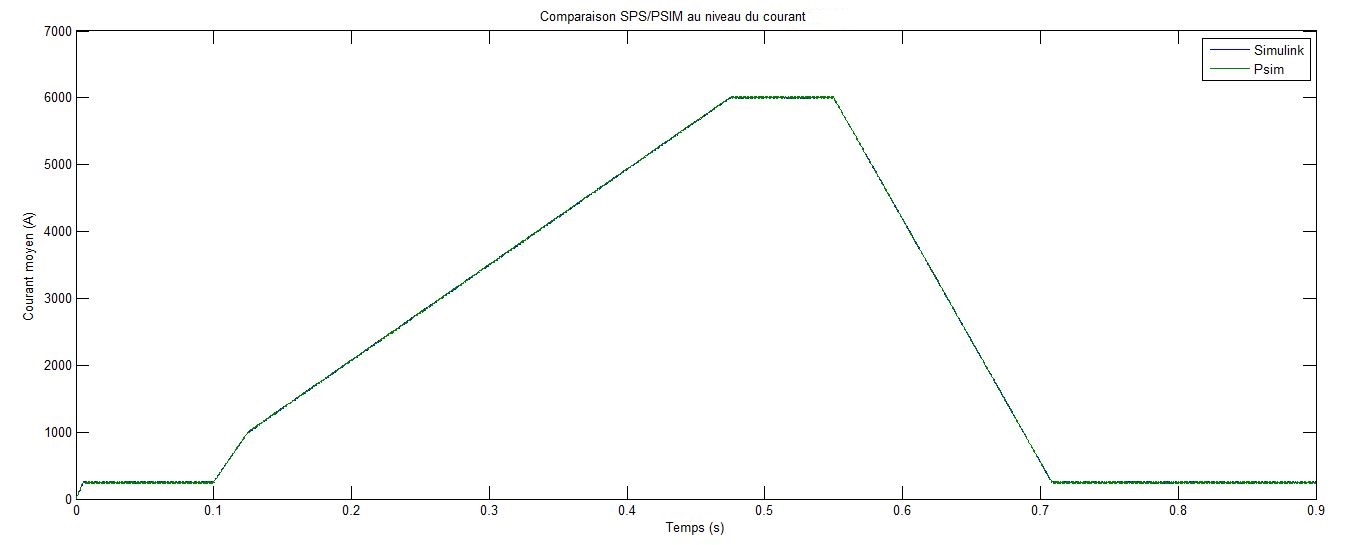
\includegraphics[scale=0.5]{comp_PSIM_SPS.jpg}
\caption{Le courant sur la charge PSIM et SPS}
\label{comp_PSIM_SPS}
\end{figure}

Lorsque le pas de calcul est de 10$^{-5}$ la fréquence de commutation observé sur le courant de la charge est de 700Hz autant sur Psim que sur simulink. Avec un pas de calcul de 10$^{-6}$ sur simulink on obtient une fréquence de commutation de 750Hz mais ce n'est pas possible d'obtenir l'information sur Psim dû à un manque de mémoire.  

\end{document}